\documentclass[a4paper,12pt]{article}

\usepackage[utf8]{inputenc}
\usepackage[T1]{fontenc}
\usepackage[czech]{babel}
\usepackage{amsmath}
\usepackage{amsfonts}
\usepackage{amssymb}
\usepackage{graphicx}
\usepackage{hyperref}
\usepackage{float}
\usepackage{hyperref}

\usepackage[a4paper]{geometry}
\geometry{verbose,tmargin=2.5cm,bmargin=2cm,lmargin=2cm,rmargin=2cm}
\usepackage{fancyhdr}
\pagestyle{fancy}

% nastaven� pisma a �e�tiny
\usepackage{lmodern}
\usepackage[T1]{fontenc}
% v�cesloupcov� tabulky
\usepackage{multirow}

% vno�en� popisky obr�zk�
\usepackage{subcaption}

% automatick� konverze EPS 
\usepackage{graphicx} 
\usepackage{epstopdf}

% odkazy a z�lo�ky


% Pozn�mky p�i p�ekladu
\usepackage{xkeyval}	% Inline todonotes
\usepackage[textsize = footnotesize]{todonotes}
\presetkeys{todonotes}{inline}{}


\title{LAR}
\author{Michal Bouda, Erik Doležal, Ondřej Váňa}
\date{\today}

\begin{document}

\maketitle

\tableofcontents

\section{Zadání}
\section{Řešení}
\subsection{Zpracování obrazu}
Zpracování obrazu děláme pomocí konvoluční neuronové sítě \href{https://docs.ultralytics.com/models/}{YOLO}. Jako vstup používáme obraz z kamery.
\subsubsection{Trénování CNN}
YOLO model jsme museli nejdříve natrénovat na rozponávání pilířů a míče. Učinili jsme tak na více než 250 obrázcích,
které jsme pořídili pomocí kamery na robotovi. Obrázky jsme ručně anotovali pomocí programu \href{https://labelstud.io/}{Label Studio}. Anotace byli poté vyexportovány ve formátu YOLO.
Pomocí Python kódu a knihovny od ultralytics jsme natrénovali model. Vyzkoušeli jsme verze v8 a 11. Zkoušeli jsme také různé rozlišení a počet epoch.
Nakonec jsme vybrali model založený na YOLO11.
\begin{figure}[H]
    \centering
    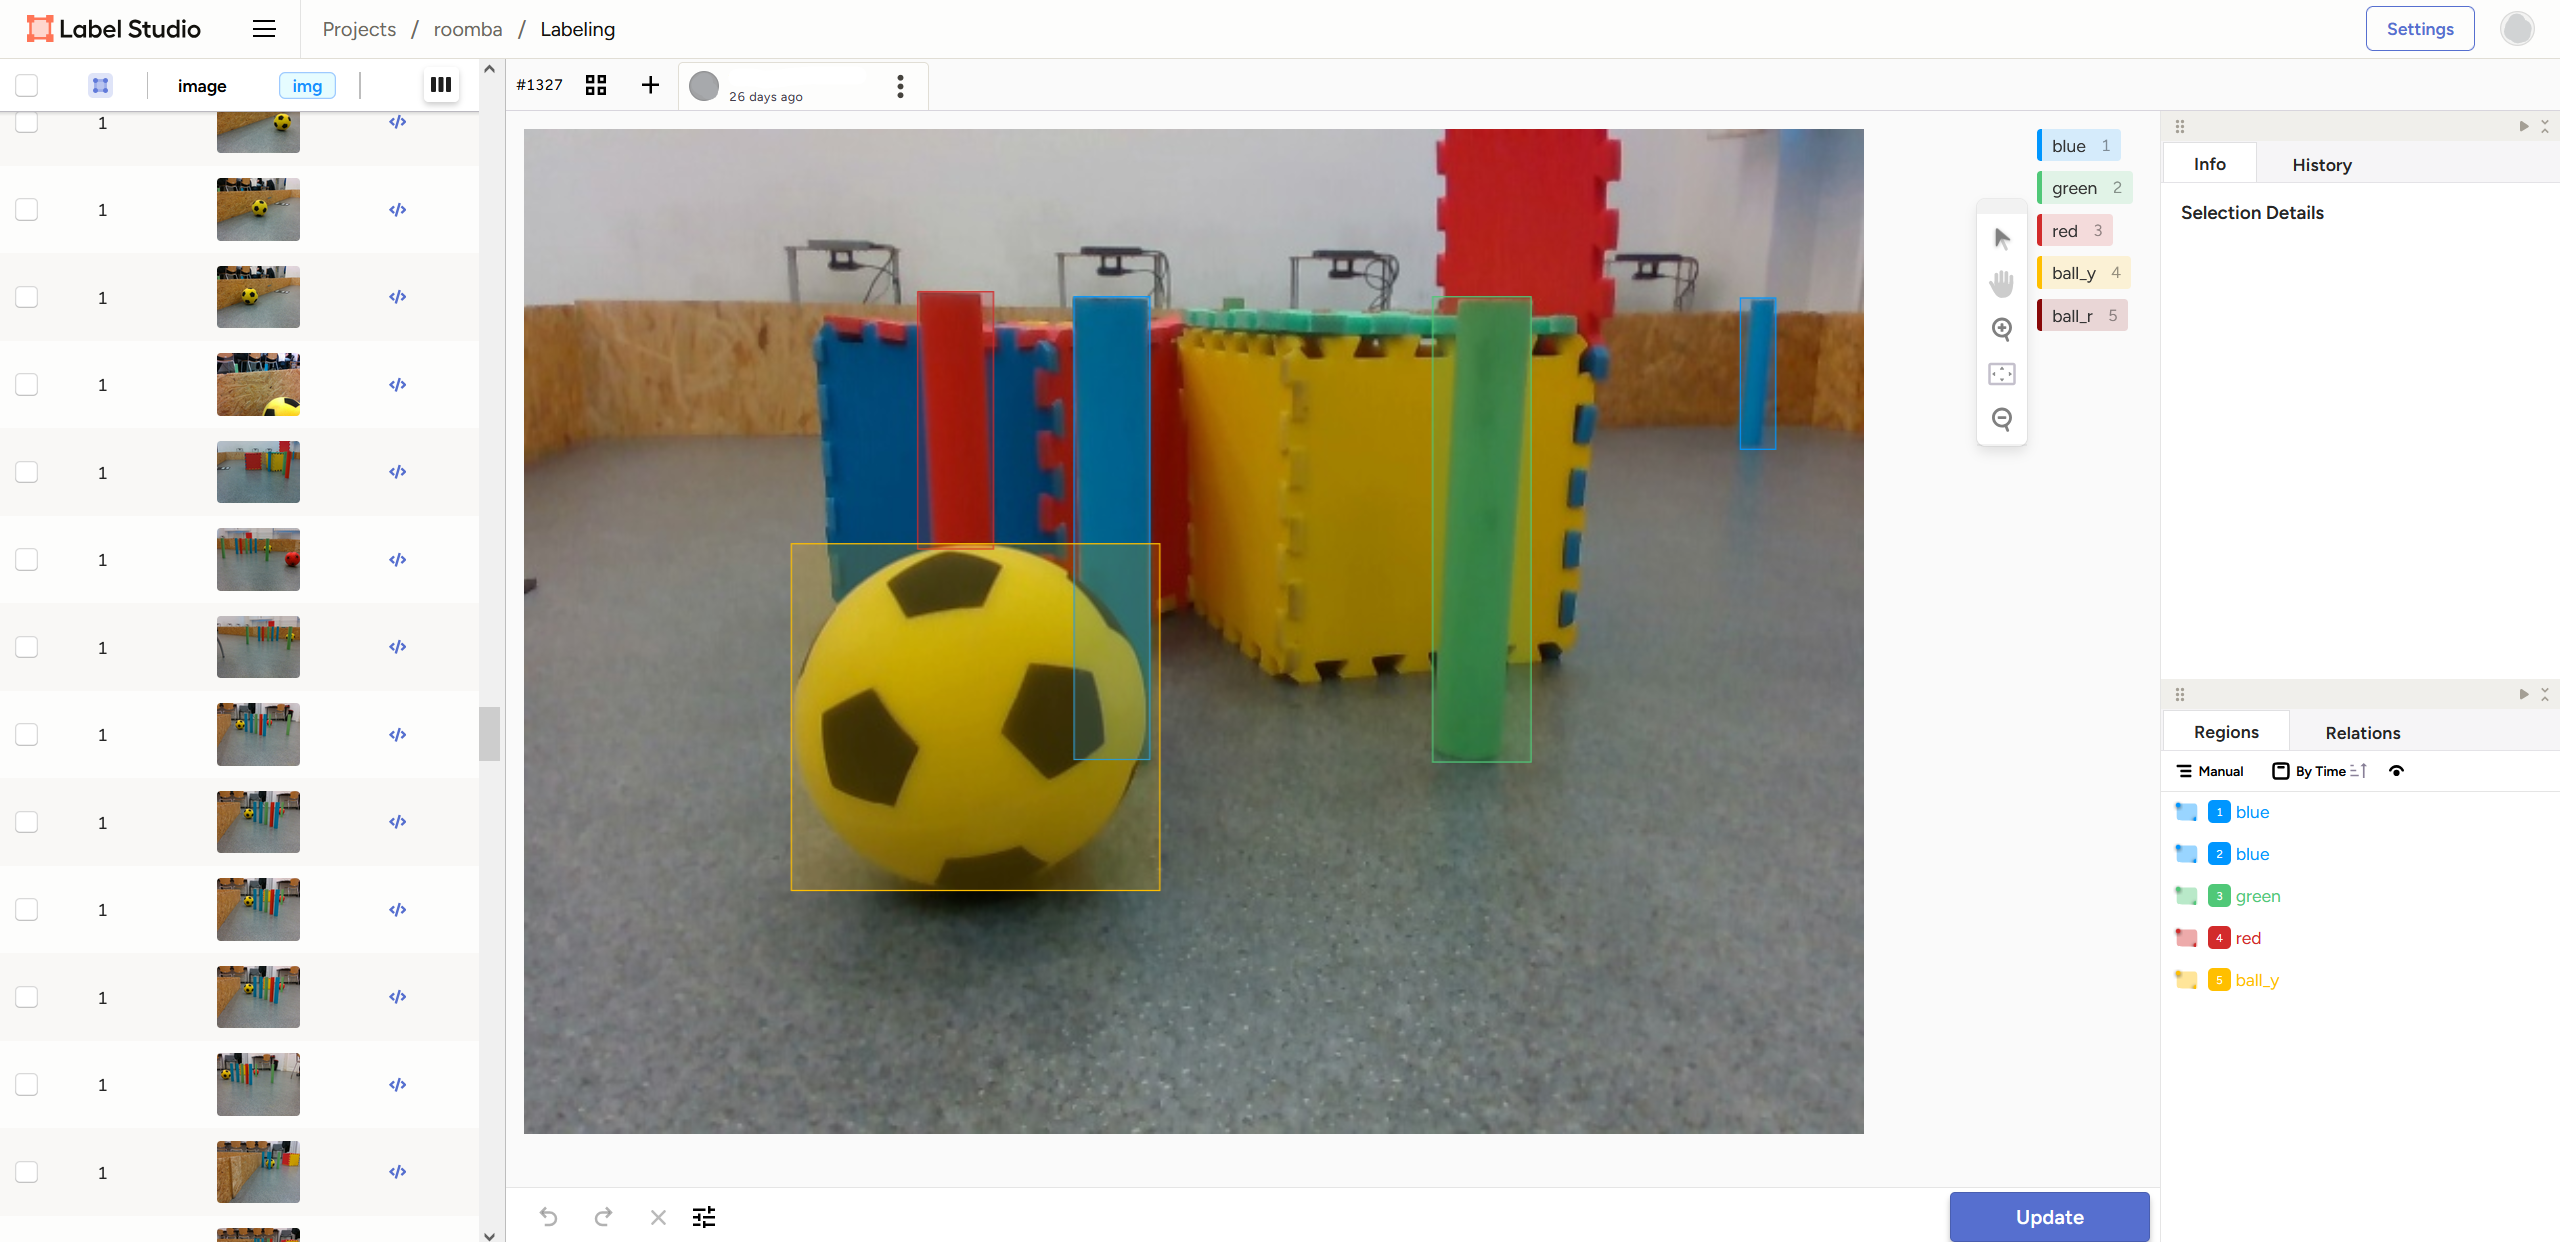
\includegraphics[width=0.8\textwidth]{pictures/label_studio.png}
    \caption{Anotování v Label Studiu}
\end{figure}

\begin{figure}[H]
    \centering
    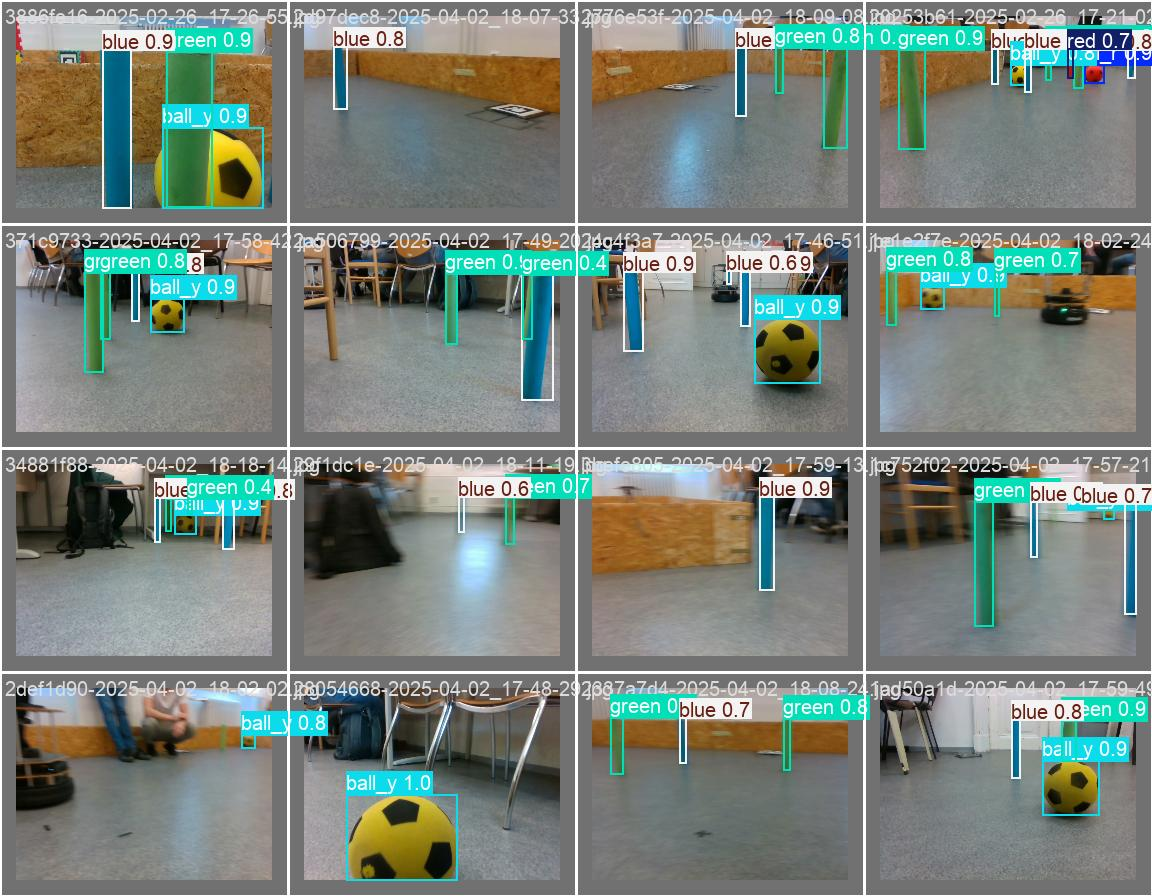
\includegraphics[width=0.7\textwidth]{pictures/rozpoznane.jpg}
    \caption{Rozpoznané objekty}
    \label{fig:example_image}
\end{figure}

\subsubsection{Rozpoznávání obrazu}
Na robotovi zajišťuje rozpoznávání class \texttt{Camera}. Třída má metodu \texttt{detect objects}, která získá obraz z kamery a vrací seznam objektů. Seznam objektů vracíme pro potřeby SLAM jako numpy array poloha x, poloha y, objekt. Poloha x, y je poloha relativně k robotovi v prostoru.

\subsubsection{Pozice objektů v prostoru}
Polohu objektů určujeme pomocí point cloudu z depth kamery. Vybereme body, které jsou ve středu obdelníku, který ohraničuje náš objekt. Z jednotlivých souřadnic je udělán medián, který je následně přenásoben maticí, která koriguje pro nahnutí kamery na robotovi. Se souřadnicí osy z již dále nepracujeme.

\subsection{SLAM}
\subsection{Plánování}
\subsection{Pohyb}
\section{Závěr}




\end{document}